\chapter{Implementation} \label{section:implementation} 
The methodology applied so far for the dataset recorded in a laboratory is to be tested on vibration signals from the industrial environment. Established guidelines for introducing a monitoring system have been described in the section on technical standards (Section~\ref{section:technical-standards}). 

We employ a slightly customized validation procedure that involves the selection of machines to be monitored, identifying positions for measurements according to technical specifications, taking preliminary readings, and developing a device capable of capturing the usual failure modes. The collection of the novel dataset is accompanied by an agreed upon schedule.

\section{Machinery for monitoring}
Three kinds of rotating machines are at disposal for vibration measurements. Those are a standing fan, scroll compressor, and water pump.

\begin{figure}[ht]
    \centering
    \begin{subfigure}[b]{0.17\textwidth}
    		\centering
        \includegraphics[width=\textwidth]{assets/design/machine-fan.jpg}
        \caption{\footnotesize Fan}
        \label{fig:machine:fan}
    \end{subfigure}
    \hfill
    \begin{subfigure}[b]{0.17\textwidth}
    		\centering
        \includegraphics[width=\textwidth]{assets/design/machine-compressor.jpg}
        \caption{\footnotesize Compressor}
        \label{fig:machine:compressor}
    \end{subfigure}
    \hfill
    \begin{subfigure}[b]{0.31\textwidth}
    		\centering
        \includegraphics[width=\textwidth]{assets/design/machine-ksb-pump.jpg}
        \caption{\footnotesize Water pump KSB}
        \label{fig:machine:pump-ksb}
    \end{subfigure}
    \hfill
    \begin{subfigure}[b]{0.31\textwidth}
    		\centering
        \includegraphics[width=\textwidth]{assets/design/machine-sigma-pump.jpg}
        \caption{\footnotesize Water pump Sigma}
        \label{fig:machine:pump-sigma}
    \end{subfigure}
    \caption{Machines dedicated for vibration measurements}
\end{figure}

\textbf{Standing fan} is model \emph{Kalorik~TKG~VT1037} (Fig.~\ref{fig:machine:fan}) and one unit is available to us. It serves as a test bed during the sensor unit development. The sensor is placed on the plastic casing at the back of the drive motor. The fan has a 45~cm diameter with 3~propellers and a power of 45~W (class~\rom{1}). It has a switch for 3 rotational speeds, which are approximately 18.5~Hz (1100~rpm), 20.4~Hz (1200~rpm), and 22~Hz (1300~rpm). Acceleration observed is $\pm 5\;\mathrm{m/s}^2$ in radial and tangential directions, and $\pm 1\;\mathrm{m/s}^2$ in axial direction.

\textbf{Scroll compressor} is model \emph{Copeland~ZR16} (Fig.~\ref{fig:machine:compressor}). Altogether two units are available in two independent air conditioning units for the data center. The compressor has 9.7~kW of power (class~\rom{1}) and rotates at 2900 rpm (48.3 Hz). Two possible measurement locations are located on the sides on top of the bearings, just above the base and above the scroll. Accelerations picked up by the sensor are $\pm 3\;\mathrm{m/s}^2$ tops.

\textbf{Water pumps} are available as 3 units in municipal drinking water pumping station. The apparatus consists of a single-stage axially split volute casing pump and an attached electric induction motor. 

The newer primary pumps with bundled wireless cloud monitoring system are two units of \emph{KSB Omega~300-560} (Fig.~\ref{fig:machine:pump-ksb}). The pumps were commissioned in 2018, and they rotate at 1493 rpm (24.9 Hz). The electric motor provides 400~kW of power (class~\rom{3}). Outer bearing on pump vibrates with acceleration of $\pm 5 \;\mathrm{m/s}^2$. 

The secondary pump is one unit named \emph{Sigma~300-OVD-600} (Fig.~\ref{fig:machine:pump-sigma}) installed in 1986. It rotates at 1485 rpm (24.75 Hz), and its electric motor has power of 450~kW. Each pump and motor have 2 bearings. Therefore, there are 4 measurement positions in total.

\begin{figure}[h]
    \centering
    \begin{subfigure}[b]{0.49\textwidth}
    		\centering
        \includegraphics[width=\textwidth]{assets/design/ksb-guard-rms.png}
        \caption{Vibration rms velocity dashboard}
    \end{subfigure}
    \hfill
    \begin{subfigure}[b]{0.49\textwidth}
    		\centering
        \includegraphics[width=\textwidth]{assets/design/ksb-guard-spectrum.png}
        \caption{Vibration spectral analysis dashboard}
    \end{subfigure}
     \caption{KSB Guard cloud monitoring for pumps}
     \label{fig:design:ksb-guard}
\end{figure}

\textbf{Complete schedule} for planned vibration data gathering on the designated machines and measurement procedure is described in Appendix~\ref{appendix:technical-docs}. In addition, we are able to export the entire historical record in hourly intervals. Logs from \textbf{KSB Guard} cloud monitoring tool contain vibration rms velocities and frequency spectra for two monitored KSB water pumps  (Figure~\ref{fig:design:ksb-guard}).


\section{Sensor hardware and drivers}
In preliminary exploratory vibration measurements of machines, the ADXL335 accelerometer is connected to BeagleBone Black microcontroller. The bandwidth, sensitivity, and sampling frequency of the makeshift solution are not appear to be adequate (Table~\ref{tab:design:hw-sensors}).

\begin{table}[ht]
\renewcommand{\arraystretch}{1.2}
\centering
\begin{tabular}{|l|l|l|}
\hline
\textbf{Accelerometer}                           & \textbf{ADXL335} & \textbf{IIS3DWB}   \\ \hline
\textbf{Vendor}                                  & Analog Devices   & STMicroelectronics \\ \hline
\textbf{Bus}                                     & Analog           & SPI                \\ \hline
\textbf{Axis}                                    & 3                & 1 or 3             \\ \hline
\textbf{Range} (g)                               & $\pm$ 3          & $\pm$ 2 to 16      \\ \hline
\textbf{Bandwidth} (kHz)                         & 0.55             & 5 - 6.3            \\ \hline
\textbf{Sensitivity}                             & 300 mV/g         & 0.061 mg/LSB       \\ \hline
\textbf{Noise density} ($\mu g / \sqrt{\mathrm{Hz}}$ rms) & 150 - 300        & 75                 \\ \hline
\textbf{Microcontroller}                         & Beaglebone Black & ESP32-PoE-ISO      \\ \hline
\textbf{CPU SoC}                                 & TI Sitara AM3358 & ESP32-WROOM-32     \\ \hline
\textbf{Output data rate} (kHz)                  & 2.5              & 26.7               \\ \hline
\textbf{ADC resolution} (bit)                    & 12               & 16                 \\ \hline
\textbf{FIFO}                                    & -                & 3 kB (512 samples) \\ \hline
\end{tabular}
\caption{Hardware parameters of previous and proposed sensor units}
\label{tab:design:hw-sensors}
\end{table}

The IIS3DWB accelerometer is a cheap enough MEMS accelerometer that approaches industrial standards for vibration monitoring. An interface capable of higher speeds is needed to store all acceleration samples. Therefore, ESP32-PoE-ISO is chosen as a microcontroller development kit because it has an SD card slot connected via SD/MMC bus. The accelerometer uses an SPI bus with a maximum speed of 10 MHz that can be connected to any physical GPIO pins. The block diagram of the designed hardware device is in Figure~\ref{fig:design:block-diagram-hw}.

\begin{figure}[h]
	\centering
	\includegraphics[width=0.9\textwidth]{assets/design/hw-block-schematic.png}
	\caption{Sensor unit hardware block diagram}
	\label{fig:design:block-diagram-hw}
\end{figure}

The drivers for necessary low-level interfaces and FAT32 filesystem are  implemented already in ESP-IDF SDK\footnote{ESP-IDF SDK: \url{https://docs.espressif.com/projects/esp-idf/en/latest/esp32/api-reference/index.html}}. The accelerometer driver is also made available by the vendor\footnote{IIS3DWB driver: \url{https://github.com/STMicroelectronics/iis3dwb-pid}}. Activity diagrams of required firmware functionality are in Appendix~\ref{appendix:technical-docs}.

\section{Preliminary measurements}
During the initial on-site inspections of machinery, we carried out preliminary measurements of vibration signals. Raw waveforms of acceleration for the fan, two different compressors, and outer bearing on a pump in three axes are plotted in Figure~\ref{fig:design:preliminary-acceleration}. The acceleration rarely exceeds 1~g. 

In frequency spectra in Figure~\ref{fig:design:preliminary-spectrum} behavior of machines can be clearly discerned, below the resonance frequency of the accelerometer (550 Hz). The compressor suspected to be faulty has stronger \nth{4} harmonic and above than the other one.


\begin{figure}[h]
    \centering
    \begin{subfigure}[b]{0.49\textwidth}
        \includegraphics[width=\textwidth]{assets/design/EDA-custom-dataset-temporal.png}
        \caption{Acceleration in $\mathrm{m/s}^2$}
        \label{fig:design:preliminary-acceleration}
    \end{subfigure}
    \hfill
    \begin{subfigure}[b]{0.49\textwidth}
        \includegraphics[width=\textwidth]{assets/design/EDA-custom-dataset-velocity.png}
        \caption{Approximate velocity in $\mathrm{mm/s}$}
        \label{fig:design:preliminary-velocity}
    \end{subfigure} 
    \caption{Temporal domain waveforms in all spatial directions with 300 ms duration at 1 s timestamp}
\end{figure} 

Figure~\ref{fig:design:preliminary-velocity} documents the effort to obtain vibration velocity (as per ISO~20186) by integration with the composite trapezoidal rule. The significant drift after integration is eliminated by subtracting the mean of the envelope constructed using cubic interpolation of peaks. Envelopes must be tweaked further to achieve more accurate values.

\begin{figure}[h]
    \centering
    \begin{subfigure}[b]{0.45\textwidth}
        \includegraphics[width=\textwidth]{assets/design/compressor-orbitals-1x.png}
		\caption{Orbital analysis of compressor's \nth{1}~harmonic frequency}
		\label{fig:design:orbital-analysis}
    \end{subfigure}
    \hfill
    \begin{subfigure}[b]{0.54\textwidth}
        \includegraphics[width=\textwidth]{assets/design/EDA-custom-dataset-spectral-X-axis.png}
        \caption{FFT with Hann window of length $2^{10}$ ($\approx$~409~ms)}
        \label{fig:design:preliminary-spectrum}
    \end{subfigure} 
    \caption{Orbital and spectral methods of vibration signal analysis}
\end{figure}

The orbital plot of the first harmonic frequency $f_{max} \pm 5\;\mathrm{Hz}$ in Figure~\ref{fig:design:orbital-analysis} allows us to check the sensor deviation out of the axis of rotation.
